\section{Experimental Paradigm}
\label{sec:experimental_paradigm}

% mlp generalization results
\begin{figure*}[h!]
    \begin{center}
        % subfigure (a)
        \begin{subfigure}[b]{0.48\textwidth}
            \begin{center}
                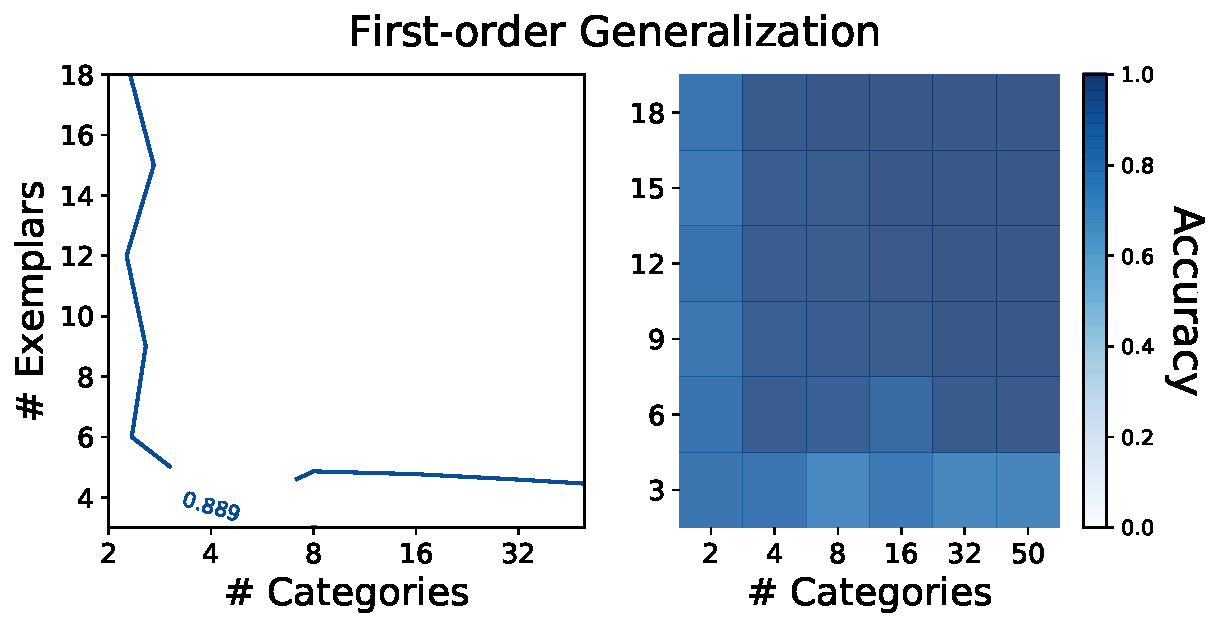
\includegraphics[width=0.98\textwidth]
                {figures/mlp_o1_acc.pdf}
            \end{center}
        \end{subfigure}
        % subfigure (b)
        \begin{subfigure}[b]{0.48\textwidth}
            \begin{center}
                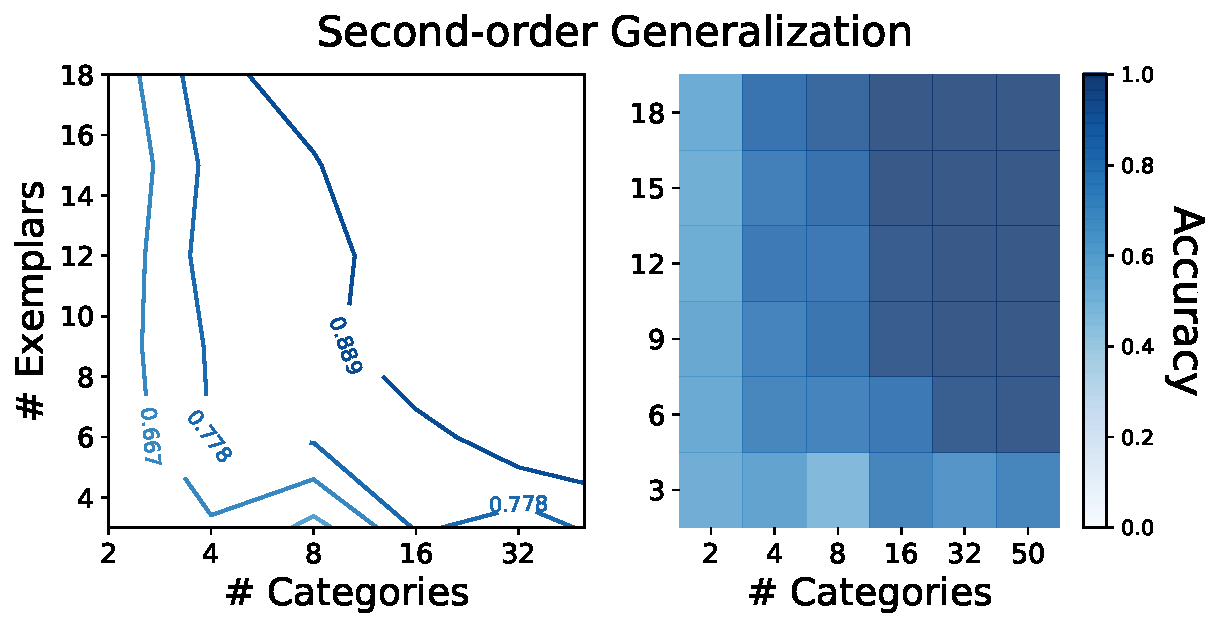
\includegraphics[width=0.98\textwidth]
                {figures/mlp_o2_acc.pdf}
            \end{center}
        \end{subfigure}
    \end{center}
    \caption{MLP generalization results for various training set sizes. Results
    show the average of 10 training runs.}
    \label{fig:mlp_gen_results}
\end{figure*}

We first set out to model the infant learning tasks described by
\cite{Smith2002} using simple neural networks. During the study, 17-month-old
children were taught the names of primitive objects over the course of 7 weeks
via weekly play sessions. Objects in the study were 3D formations constructed of
various materials; each object contained a specific shape, color
and texture (material), and the names of the objects were organized stricly
by shape. During the weekly sessions, children played around with each object
while an adult announced the name of the object that they were playing with
repeatedly. By the end of the study, the children subjects had learned the
shape bias--i.e., they had formed the generalization that only objects with
the same shape have the same name. A control group of children, whom did not
partake in the play sessions, did not form the same generalization.

To model this study, we use artificial object datasets designed to
mimick the training data presented to the children subjects. We first perform
our computational experiments with categorical bit-vector data, followed by
RGB images. The details of these two data formats and their corresponding network
architectures are described in the succeeding two sections, respectively. Each object sample is
assigned a shape, texture and color value. We train simple neural networks to
classify the shape of each object, providing labels that mimick
those provided to the children. Training is performed for various dataset sizes,
varying both the number of categories and the number of exemplars of each
category provided to the network. We evaluate the generalization capabilities
of the network for each training set size using two generalization tests
modeled after the two tests of \cite{Smith2002}.

{\bf1. First-order generalization test}: For the first-order generalization
test, infants are first presented with a baseline object that they have seen and
played with during training. Then, they are presented with three novel objects
that have not been seen before: one that matches the baseline in shape, one
that matches in color, and one that matches in texture. For each match,
the other two stimulus aspects are novel. The infants are asked to select
which of the three comparison objects share the same name as the baseline.
Performance is measured as the fraction of trials in which the child
selected the correct object, i.e. the shape match. \cite{Smith2002} propose
that children who display the first-order generalization capability have taken the first
step in the development of the shape bias: they have learned to attend to
shape when identifying exemplars of familiar object categories.
To simulate this test, we create an evaluation set containing groupings of four samples: a baseline, a
shape match, a color match, and a texture match. We find which of the three
samples the network thinks to be most similar by evaluating the cosine similarity
\footnote{Near-identical results were observed using Euclidean distance.}
using features at the last hidden layer of the model. Accuracy is defined as
the fraction of groupings for which the model chose the correct (shape-similar)
object.

{\bf2. Second-order generalization test}: For the second-order generalization
test, infants are first presented with a baseline object that is novel in shape,
color and texture. From there, the trial proceeds similarly to those of the
first-order: a shape match, color match and texture match are presented,
and the child must select which object she believes to share a name with the
baseline. All shapes, colors and textures are novel to the child in this test.
\cite{Smith2002} propose that children who display the second-order
generalization capability have taken one step further beyond the first-order
test in the development of the shape bias. These children have not only learned
to categorize a handful of object cateogories by shape, but they have induced
that shape is a useful feature in general when categorizing objects. This
induction, it was shown, is useful for vocabulary development. We simulate
the second-order test with artificial object stimuli similarly as done in the
first-order case, again using last hidden layer features to quantify model similarity
scores.

We hold a novel set of shapes, colors and textures to be used for the
generalization tests in our experiments. Accuracy over 2000 test trials is
recorded as the performance metric for each generalization.

